\cleardoublepage
\section{Mathematical model}
\label{sec:mathMod}
In the present work, the air-flow in the inhabited area is investigated together with the transport of the pollution emerging on the main road. The chosen simulation approach is a segregated one: 
\begin{inparaenum}[(i)]
    \item a steady state velocity field is pre-calculated using Navier-Stokes equations, and
    \item it is used in scalar transport equation to simulate advancement of the pollution. 
\end{inparaenum}

The present section describing the used mathematical model is structured as follows: 
\begin{inparaenum}[(i)]
    \item a model geometry and a computational mesh generation are presented,
    \item used boundary conditions are summarized and
    \item the governing equations are briefly outlined.
\end{inparaenum}

\subsection{Model geometry generation and boundary conditions}
\label{subsec:geomGen}
As stated, the air flow and the spread of the pollution in the inhabited area is of an interest. A studied part of the city is $L_{\mathrm{l}} = 500$\,m long, $L_{\mathrm{w}} = 500$\,m wide, and the highest building is $L_{\mathrm{h}} = 105$\,m tall. The available \textit{stl} file together with its dimensions and the orientation in the chosen Cartesian coordinate system is depicted in Figure~\ref{fig:geom1}.

\begin{figure}[htpb]
    \begin{tikzpicture}[
            axPic/.pic={
                \draw[->,-triangle 45] (0,0) -- (-0.,0.8)  node (ysign) [pos=1,right] {$z$};
                \draw[->,-triangle 45] (0,0) -- (0.5,0.33) node (xsign) [pos=1,right] {$x$};
                \draw[->,-triangle 45] (0,0) -- (-0.6,0.2) node (zsign) [pos=1,left] {$y$};
            }]
            
        \node (obr) {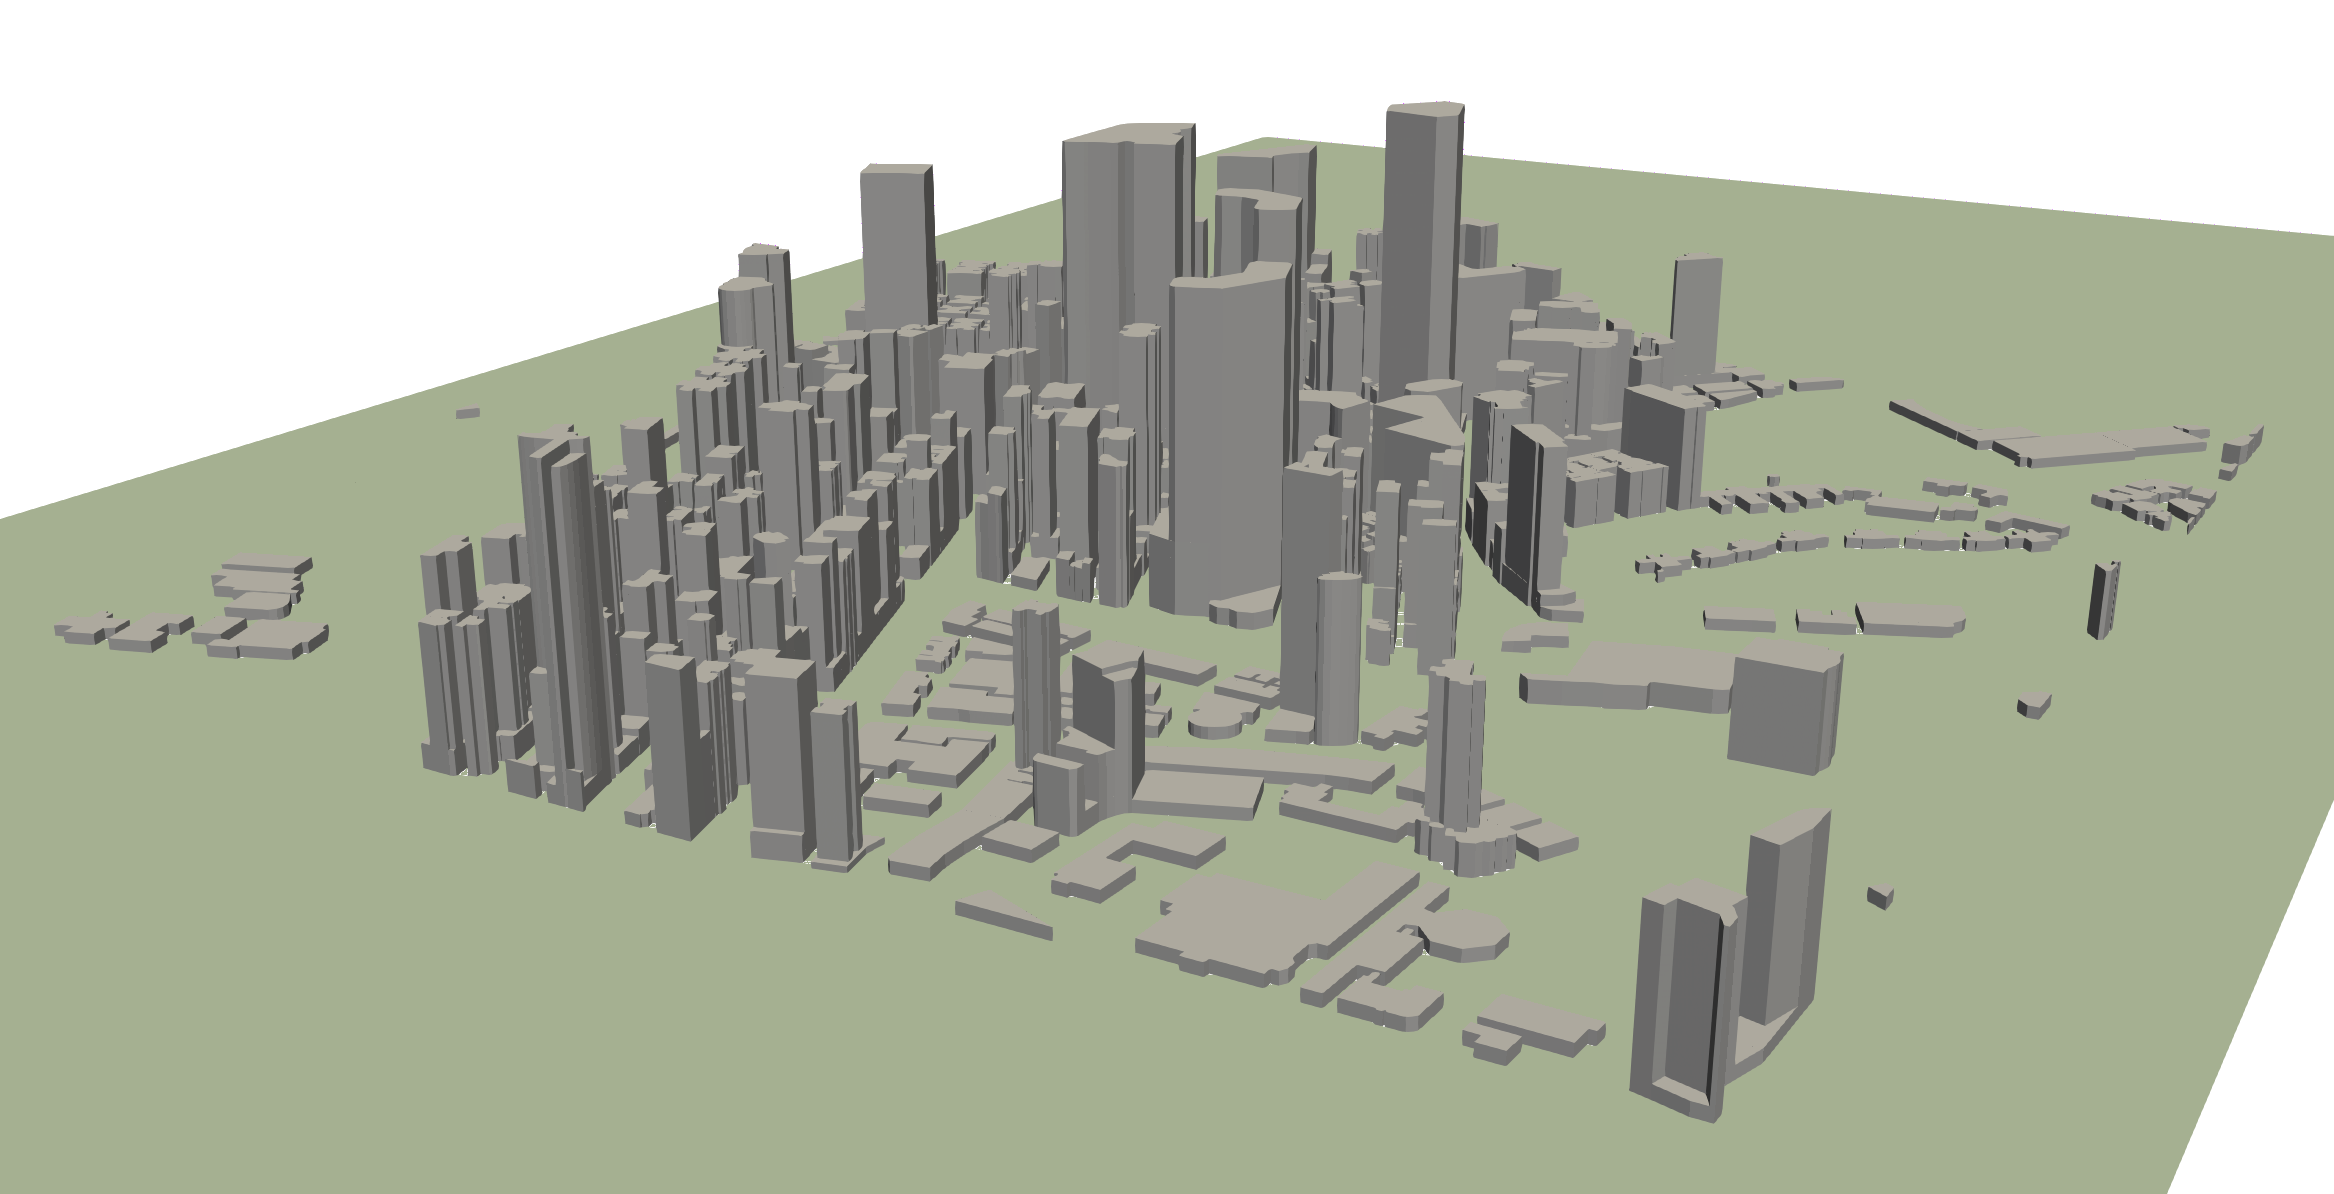
\includegraphics[width=0.95\textwidth]{01_images/geometry/geom1.png}};
        \draw[latex-latex, color=yellow, line width = 0.005\textwidth] ([yshift=0.07\textwidth,xshift=0-0.015\textwidth]obr.east) -- ([xshift=0.24\textwidth,yshift=0.025\textwidth]obr.south);
        \node at (obr.south east) [xshift=0-0.1\textwidth,yshift=0.15\textwidth] {500\,m};
        \draw[latex-latex, color=yellow, line width = 0.005\textwidth] ([xshift=0.2\textwidth,yshift=0.025\textwidth]obr.south) -- ([xshift=0.012\textwidth,yshift=0-0.03\textwidth]obr.west);
        \node at (obr.south) [xshift=0-0.2\textwidth,yshift=0.12\textwidth] {500\,m};
        \draw[-latex, color=yellow,line width = 0.005\textwidth] ([xshift=0.11\textwidth,yshift=0.09\textwidth]obr.center) -- ([xshift=0.113\textwidth,yshift=0-0.055\textwidth]obr.north);
        \node at (obr.north) [xshift=0.155\textwidth,yshift=0-0.083\textwidth] {105\,m};
        \draw (-6.5,-3.2) pic[solid] {axPic};
    \end{tikzpicture}
    \caption{Studied city geometry (used \textit{stl} file) with its dimensions and chosen Cartesian coordinate system.}
    \label{fig:geom1}
\end{figure}

\paragraph{Computational mesh} Computational mesh was prepared using the OpenFOAM \texttt{blockMesh} and \texttt{snappyHexMesh} utilities. The computational domain dimensions were determined based on the review by \citet{Pantusheva22}. In particular, we introduce both upstream, and downstream buffers in front of, and behind the city, which are in order $L_{\mathrm{CFDu}} = 5\,L_{\mathrm{h}}$, and $L_{\mathrm{CFDd}} = 10\,L_{\mathrm{h}}$ long. Furthermore, the computational domain is $L_{\mathrm{CFDh}} = 6\,L_{\mathrm{h}}$ high. The $y$-normal slices cut in the middle of the used computational mesh are shown in Figure~\ref{fig:mesh1}. Note the grading of the computational mesh in the $z$-direction, and its refinement in the vicinity of the city. 

\begin{figure}[htpb]
    \begin{tikzpicture}
        \node (obr) {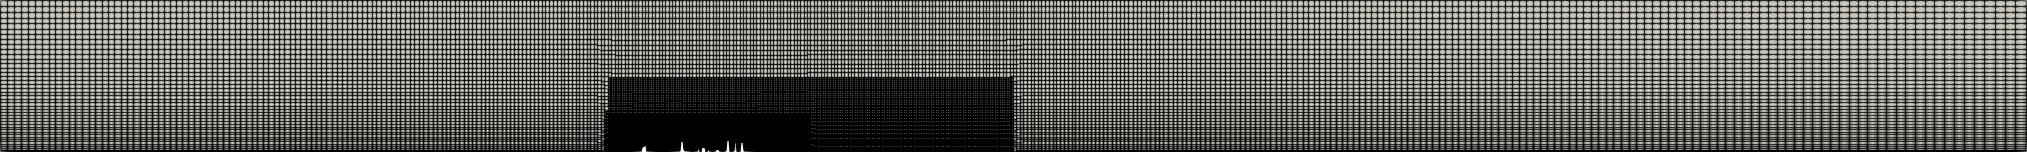
\includegraphics[width=0.95\textwidth]{01_images/geometry/mesh1.png}};
        \draw[latex-latex, line width=0.002\textwidth] ([xshift=0.005\textwidth]obr.north west)--([xshift=0-0.19\textwidth]obr.north);
        \node at (obr.north) [anchor = south west,xshift=0-0.42\textwidth] {$L_{\mathrm{CFDd}}\,=\,5\,L_{\mathrm{h}}$};
        \draw[latex-latex, line width=0.002\textwidth] ([xshift=0-0.12\textwidth]obr.north)--([xshift=0-0.005\textwidth]obr.north east);
        \node at (obr.north) [anchor = south west,xshift=0.08\textwidth] {$L_{\mathrm{CFDu}}\,=\,10\,L_{\mathrm{h}}$};
        \draw[latex-latex, line width=0.002\textwidth] ([yshift = 0-0.005\textwidth] obr.north west) -- ([yshift=0.005\textwidth] obr.south west);
        \node at (obr.west) [rotate=90,anchor = south] {$6\,L_{\mathrm{h}}$};
        \node (detail1) at (obr.south west) [inner sep=0,yshift=0-0.01\textwidth,anchor = north west,xshift=0.008\textwidth] {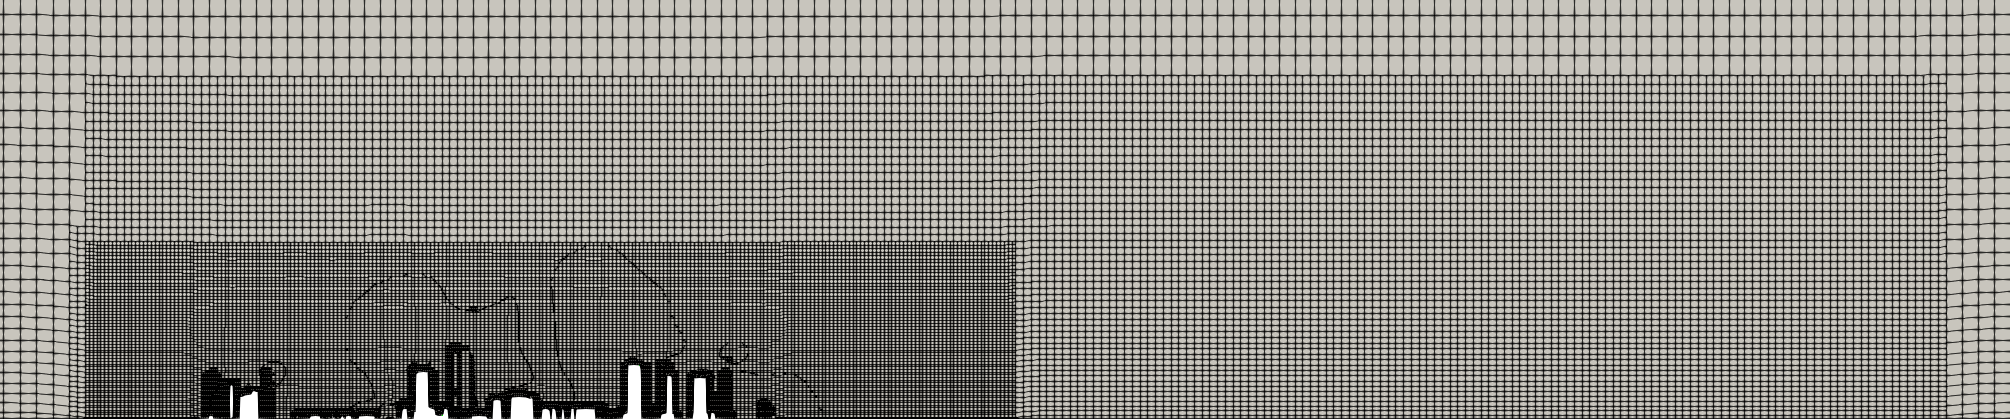
\includegraphics[width=0.45\textwidth]{01_images/geometry/mesh2.png}};
        \draw[line width = 0.003\textwidth, color=yellow!20!orange] (detail1.north west) -- (detail1.north east)--(detail1.south east) -- (detail1.south west) -- (detail1.north west);
        \draw[line width=0.003\textwidth, color=yellow!20!orange] ([xshift=0.005\textwidth,yshift=0.007\textwidth]obr.south)--([xshift=0-0.2\textwidth,yshift=0.007\textwidth]obr.south) -- ([xshift=0-0.2\textwidth,yshift=0.05\textwidth]obr.south)--([xshift=0.005\textwidth,yshift=0.05\textwidth]obr.south) --([xshift=0.005\textwidth,yshift=0.007\textwidth]obr.south);
        \node (detail2) at (obr.south east) [inner sep = 0, yshift = 0-0.01\textwidth,anchor = north east,xshift=0- 0.008\textwidth] {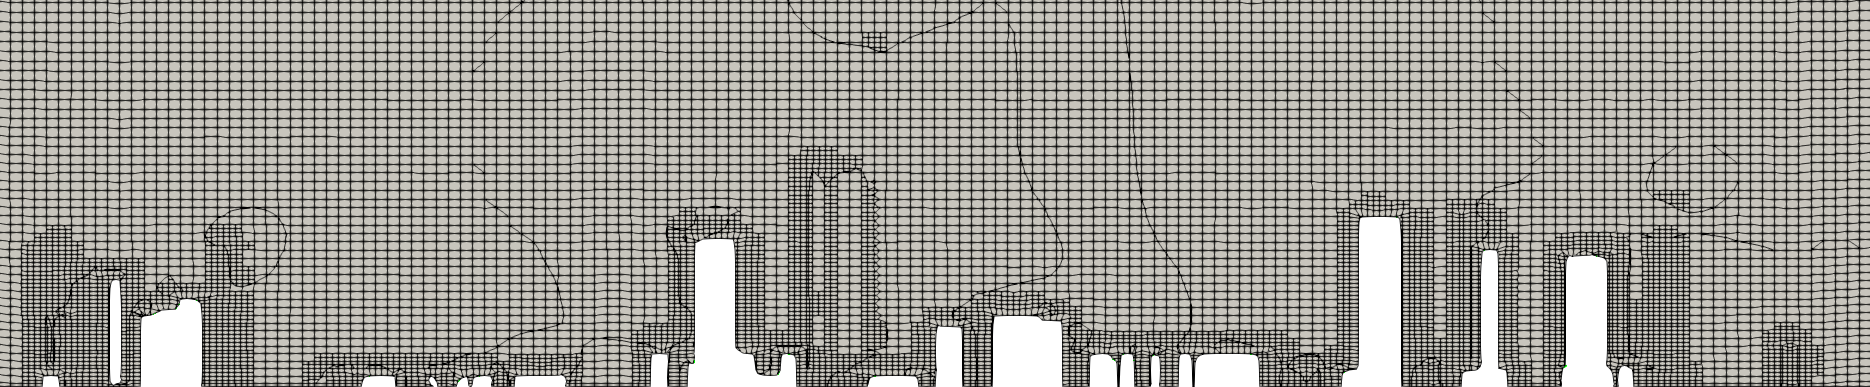
\includegraphics[width=0.45\textwidth]{01_images/geometry/mesh3.png}};
        \draw[line width = 0.003\textwidth, color=blue!70] (detail2.north west) -- (detail2.north east)--(detail2.south east) -- (detail2.south west) -- (detail2.north west);
        \draw[line width=0.003\textwidth, color=blue!70] ([xshift=0-0.12\textwidth,yshift=0.007\textwidth]obr.south)--([xshift=0-0.181\textwidth,yshift=0.007\textwidth]obr.south) -- ([xshift=0-0.181\textwidth,yshift=0.022\textwidth]obr.south)--([xshift=0-0.12\textwidth,yshift=0.022\textwidth]obr.south) --([xshift=0-0.12\textwidth,yshift=0.007\textwidth]obr.south);
    \end{tikzpicture}
    \caption{$y$-normal slices through the half of the computational mesh.}
    \label{fig:mesh1}
\end{figure}

\paragraph{Boundary conditions} The model behavior in the computational domain ($\Omega$) is described by partial differential equations outlined in the following subsection~\ref{subsec:govEq} (\nameref{subsec:govEq}). However, these need to be supplied with the consistent boundary conditions on the $\Omega$ boundary, $\partial\Omega$. As depicted in Figure~\ref{fig:bc}, the computational domain boundary is split into 
\begin{inparaenum}[(i)]
    \item \textit{inlet} ($\partial\Omega_{\mathrm{i}}$),
    \item \textit{outlet} ($\partial\Omega_{\mathrm{o}}$),
    \item \textit{ground} ($\partial\Omega_{\mathrm{g}}$),
    \item \textit{sides} ($\partial\Omega_{\mathrm{s}}$), and
    \item \textit{top} ($\partial\Omega_{\mathrm{t}}$).
\end{inparaenum}
 
\begin{figure}[htpb]
    \begin{tikzpicture}
        \node (obr) {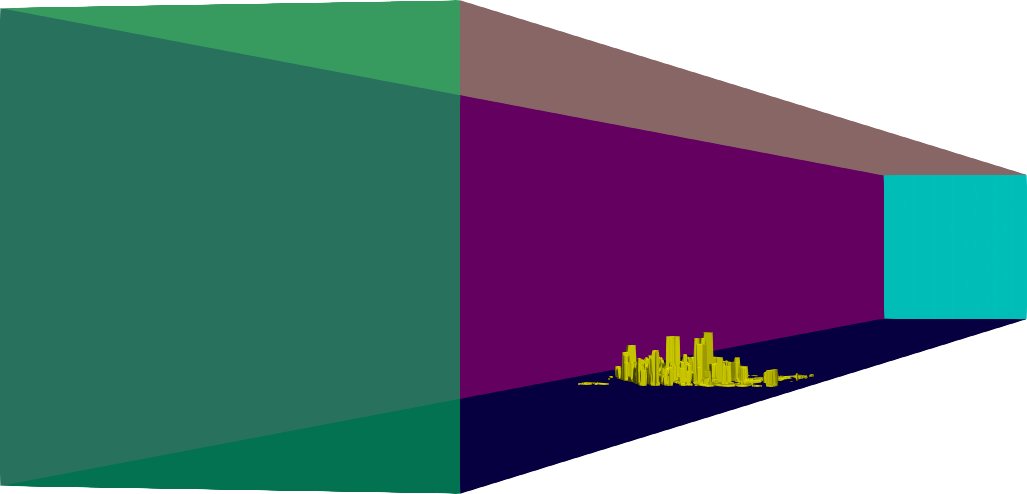
\includegraphics[width=0.6\textwidth]{01_images/geometry/bc1.png}};
        \node (inlet) at ([{shift={(0.05\linewidth,0-0.068\linewidth)}}]obr.north east) [draw,color=in,fill=in,minimum width=0.03\linewidth,minimum height=0.03\linewidth] {};
        \node [name=wall, at=(inlet.east),anchor=west]{{$\partial\Omega_{\mathrm{i}}$}};
        \node (outlet) at (inlet.south) [draw,color=out,fill=out,minimum width=0.03\linewidth,minimum height=0.03\linewidth,anchor=north,yshift=0-0.01\textwidth] {};
        \node[name=wall, at=(outlet.east),anchor=west]{{$\partial\Omega_{\mathrm{o}}$}};
        \node (ground) at (outlet.south) [draw,color=city,fill=city,minimum width=0.03\linewidth,minimum height=0.03\linewidth,anchor=north,yshift=0-0.01\textwidth] {};
        \node (ground2) at (ground.east) [draw,color=lw,fill=lw,minimum width=0.03\linewidth,minimum height=0.03\linewidth,anchor=west,xshift=0.01\textwidth] {};
        \node[name=wall, at=(ground2.east),anchor=west]{{$\partial\Omega_{\mathrm{g}}$}};
        \node (sides) at (ground.south) [draw,color=fb,fill=fb,minimum width=0.03\linewidth,minimum height=0.03\linewidth,anchor=north,yshift=0-0.01\textwidth] {};
        \node[name=wall, at=(sides.east),anchor=west]{{$\partial\Omega_{\mathrm{s}}$}};
        \node (top) at (sides.south) [draw,color=top,fill=top,minimum width=0.03\linewidth,minimum height=0.03\linewidth,anchor=north,yshift=0-0.01\textwidth] {};
        \node[name=wall, at=(top.east),anchor=west]{{$\partial\Omega_{\mathrm{t}}$}};
    \end{tikzpicture}
    \caption{Boundaries of the computational domain.}
    \label{fig:bc}
\end{figure}

Used boundary conditions are utilized from~\cite{kadaverugu21,Pantusheva22} and summarized in Table~\ref{tab:bc}. 

\begin{table}[htbp]
    \caption{Used boundary conditions.}
    \label{tab:bc}
    \centering
    {
    \begin{tabular}{lccccccccc}
        \hline
        variable & $\Omega_{\mathrm{i}}$ & $\Omega_{\mathrm{o}}$ & $\Omega_{\mathrm{g}}$ &  $\Omega_{\mathrm{s}}$ & $\Omega_{\mathrm{t}}$ \\
        \hline
        $\bm{u}$ & fixedValue & inletOutlet & noSlip & slip & slip\\
        $p$ & zeroGrad & totalPressure & zeroGrad & zeroGrad & zeroGrad\\
        $k$ & turbIntKinEngInlet & zeroGrad & kqRWallFunction & zeroGrad & zeroGrad\\
        $\varepsilon$ & turbMixDissRateInlet & zeroGrad & epsWallFunction & zeroGrad & zeroGrad\\
        $\nu_{\mathrm{t}}$ & fixedValue & zeroGrad & nutkWallFunction & zeroGrad & zeroGrad\\
        $y_{\mathrm{P}}$ & zeroGrad & zeroGrad & fixedValue & zeroGrad & zeroGrad\\
        \hline
    \end{tabular}
    }
\end{table}

\subsection{Governing equations}
\label{subsec:govEq}
The description of the chosen governing equations can be split into two parts, 
\begin{inparaenum}[(i)]
    \item air-flow governing equations, and
    \item the pollution 
\end{inparaenum}

\subsection{Developed OpenFOAMCase python class documentation}
\label{subsec:ofCaseClass}
